\chapter{Design of the application}

This section aims to explain the architecture and design choices made for the demonstration application.

The code for the program described is available at github\footnote{ \url{https://github.com/Rymdsnigel/thesis-demo}}.

\section{Overall architecture}
The demonstration program consists of a server that continously accepts connecting clients and a client that connects with the server. An arbitrary number of clients can run and connect to the server at the same time. 

\begin{figure}[h!]
\centering
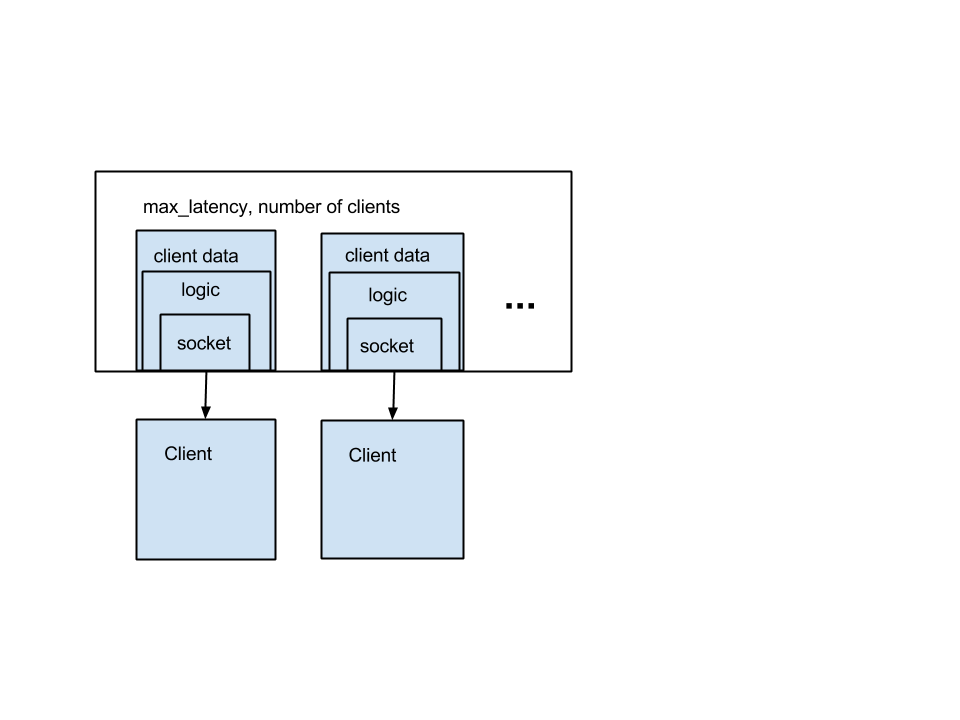
\includegraphics[width=1.0\textwidth]{figures/arch.png}
\caption{Overall architecture of the system.}
\end{figure}


\section{Why the Client-Server approach?}
The client-server approach was chosen, as opposed to choosing a master among the clients, since there was a need to both generate and distribute specific events from a central source.

\section{Events}
\label{events}
Both the client and the server create events that will be parsed to JSON and sent either from the server to the clients or from the client to the server. The server produces render events on input from the pygame window, sync events on key input from the pygame window and latency update events as a reply to sych events from the client, while the client only produces sync events as reply to the server sync events. All three different types of events have an event type, an integer that identifies the type of event.

The content of the sync event and the latency update event will be explained in chapter 4. The three different types of events are shown below. 

\begin{tabular}{ l | r }
  latency\_update\_event \\
  \hline                        
  "event\_type" & 0 \\
  "latency" & latency \\
  "max\_latency" & max latency \\
  \hline  
\end{tabular}

\begin{tabular}{ l | r }
  sync\_event \\
  \hline                        
  "event\_type" & 1 \\
  "recieved\_at" & recieved at \\
  "sent\_at" & sent at \\
  "delta" & delta \\
  "client\_id" & client id \\
  \hline  
\end{tabular}

\begin{tabular}{ l | r }
  render\_event \\
  \hline                        
  "event\_type" & 2 \\
  "id" & id \\
  "channel" & channel \\
  "data\_id" & data id \\
  "data\_val" & data val \\
  "timestamp" & timestamp \\
  "reserved" & reserved \\
  \hline  
\end{tabular}

%\begin{figure}[h!]
%\centering
%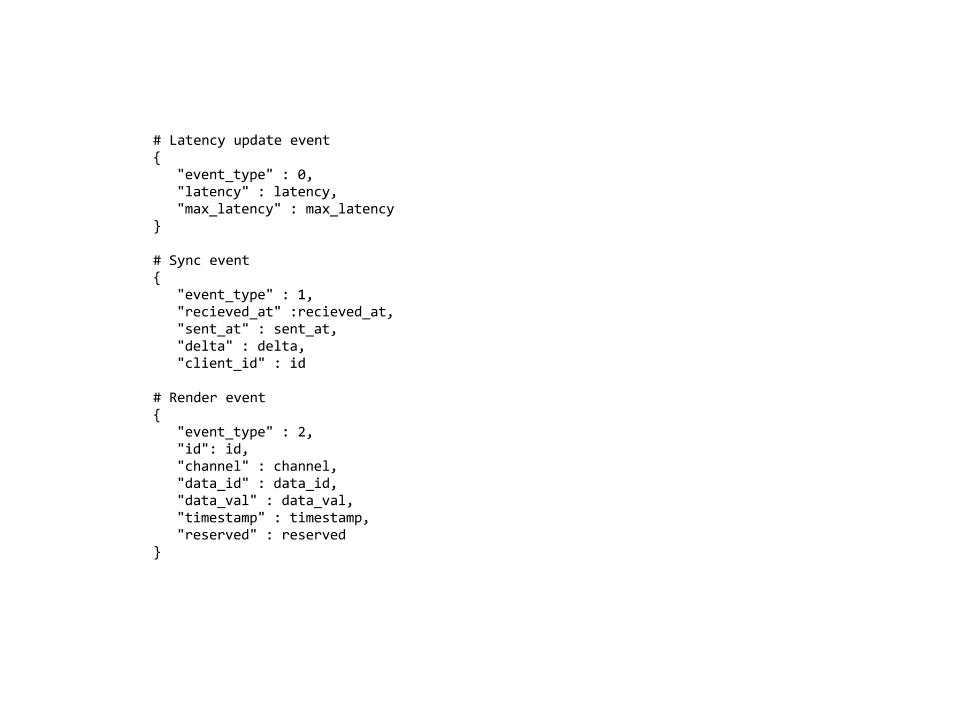
\includegraphics[width=1.3\textwidth]{figures/events.png}
%\caption{Event types.}
%\label{events}
%\end{figure}

\section{Event queues}
Both the server and the clients have event queues, when they create an event they place it in their queue. Messages are then polled from the queue and sent one at the time. This works in the same way on the clients and the server and the purpose is to avoid blocking other threads by sending data.

\section{Messaging}
The server and the clients send and recieve JSON, the json is created using simplejson library functions, dumps() for creating JSON from a dict and loads() for unpacking the dict from JSON. The functions for generating the dicts that will be sent as the messages are specified in event.py, and the specified dicts are shown in the section about events \footnote{\ref{events}}. 

The choice of JSON for messaging, rather than using pickle, cpickle or XML was made due to JSONs speed of reading and writing \footnote{\url{http://kovshenin.com/2010/pickle-vs-json-which-is-faster/}, Kovshenin} and to support future flexibility in language since pickle and cpickle is python-specific. 

\section{Communication}

\subsection{Protocols}
The choice of TCP-sockets as opposed to UDP-sockets was made at an early stage of development. Although UDP is typically the ideal choice for time critical applications, customizing the needed control mechanisms would be outside the scope of this thesis. 

The choice of TCP presented proved to be problematic when it was discovered that TCP:s message buffering, using Nagels algoritm, generated a general delay in messaging, a delay of 20 ms both from the server as from the clients. This was discovered by measuring the delays of the application over localhost, where network delays should be close to 0. This issue also resulted in that more than one json object could be put on the queue of recieved events, which lead to a json-parsing error when trying to load the objects. These errors and the buffer delays were removed by disabling Nagels algorithm\footnote{\url{http://stackoverflow.com/questions/8617809/unstable-tcp-receive-times}} by setting the nodelay flag on the socket.

%source nagels algoritm

\begin{figure}[h!]
\centering
\texttt{self.s.setsockopt(socket.IPPROTO\_TCP, socket.TCP\_NODELAY, 1)}
\caption{Setting the nodelay flag on the socket}
\end{figure}

\subsection{Sockets}
The demo server communicates with the clients via gevent sockets since the sockets need to be threaded in order to not block the other processes. 

% ref to section about greenlets.
% explaining gevent sockets as opposed to regular sockets. 

\subsection{Replacing the networklayer}
Functional cohesion has been strived for, in order to make the part of the code pertaining to transport easily replaced by for example an implementation using UDP or implementation of a ready solution such as redis. Though this has not been entirely accomplished %in which ways is it not.






\section{Threading}
\label{sec:threading}

Both the server and the client have to achieve concurrency. This is done by letting both the TransportServer and the TransportClient inherit from gevent Greenlets. 
Greenlets are pseudothreads that share the same OS-thread, and cooperatively multitask. Because it is cooperative, the threads must release control of critical operations to avoid blocking other threads. 

\section{Animations}

For animations as well as server input Pygame was chosen, because of its simplicity to work with. Pygame is built on SDL\footnote{\url{http://www.pygame.org/wiki/about}} and is a Python library for game development.

\subsection{Tweening}

Since it is necessary to be able to manipulate the time when every client performs a specific animation one of the first steps was to make the animations time dependent and independent from framerate. This is solved in the Tween class. The Tween class has two functions for generating input for the animations. This generated input can be used for, for example, deciding the position of an object or the color of a part of an object. 

In every frame drawn on the client the current time is sent to the animation's step function in the client's Tween instance. The animation saves the current time between frames and can then calculate the delay between two frames (delta). The animation then uses the delta value to interpolate between the start and the end values, ensuring that the animation runs for a set amount of time. This way the time of the animation can be manipulated by giving the Tween functions a value for current time that is in sync with the other clients. 

Making the animations time dependant by timestepping is a major part of the chosen solution for synchronizing the animations presented in this thesis. 

The functions for generating data for the animations are in the Tween class, see appendix B.  




